\documentclass[a4paper]{book}%
%%%%%%%%%%%%%%%%%%%%%%%%%%%%%%%%%%%%%%%%%
% Professional Newsletter Template
% Structural Definitions File
% Version 1.0 (09/03/14)
%
% Created by:
% Vel (vel@latextemplates.com)
% 
% This file has been downloaded from:
% http://www.LaTeXTemplates.com
%
% License:
% CC BY-NC-SA 3.0 (http://creativecommons.org/licenses/by-nc-sa/3.0/)
%
%%%%%%%%%%%%%%%%%%%%%%%%%%%%%%%%%%%%%%%%%

%----------------------------------------------------------------------------------------
%	REQUIRED PACKAGES
%----------------------------------------------------------------------------------------

\usepackage{graphicx} % Required for including images
\usepackage{microtype} % Improved typography
\usepackage{multicol} % Used for the two-column layout of the document
\usepackage{booktabs} % Required for nice horizontal rules in tables
\usepackage{wrapfig} % Required for in-line images
\usepackage{float} % Required for forcing figures not to float with the [H] parameter

%------------------------------------------------
% Fonts

\usepackage{charter} % Use the Charter font as the main document font
\usepackage{courier} % Use the Courier font for \texttt (monospaced) only
\usepackage[T1]{fontenc} % Use T1 font encoding
\usepackage{lmodern}

%------------------------------------------------
% List Separation

\usepackage{enumitem} % Required to customize the list environments
\setlist{noitemsep,nolistsep} % Remove spacing before, after and within lists for a compact look

%------------------------------------------------
% Figure and Table Caption Styles

\usepackage{caption} % Required for changing caption styles
\captionsetup[table]{labelfont={bf,sf},labelsep=period,justification=justified} % Specify the table caption style
\captionsetup[figure]{labelfont={sf,bf},labelsep=period,justification=justified, font=small} % Specify the figure caption style
\setlength{\abovecaptionskip}{10pt} % Whitespace above captions

%------------------------------------------------
% Spacing Between Paragraphs

\makeatletter
\usepackage{parskip}
\setlength{\parskip}{6pt}
\newcommand{\@minipagerestore}{\setlength{\parskip}{6pt}}
\makeatother

%----------------------------------------------------------------------------------------
%	PAGE MARGINS AND SPACINGS
%----------------------------------------------------------------------------------------

\textwidth = 7 in % Text width
\textheight = 10 in % Text height
\oddsidemargin = -18pt % Left side margin on odd pages
\evensidemargin = -18pt % Left side margin on even pages
\topmargin = -36pt % Top margin
\headheight = 0pt % Remove the header by setting its space to 0
\headsep = 0pt % Remove the space between the header and top of the page
\parskip = 4pt % Space between paragraph
\parindent = 0.0in % Paragraph indentation
\pagestyle{empty} % Disable page numbering

%----------------------------------------------------------------------------------------
%	COLORS
%----------------------------------------------------------------------------------------

\usepackage[dvipsnames,svgnames]{xcolor} % Required to specify custom colors

\definecolor{altncolor}{rgb}{.8,0,0} % Dark red
%\definecolor{altncolor}{rgb}{.2,.4,.8} % Dark blue
%\definecolor{altncolor}{rgb}{.84,.16,.16} % Red

\usepackage[colorlinks=true, linkcolor=altncolor, anchorcolor=altncolor, citecolor=altncolor, filecolor=altncolor, menucolor=altncolor, urlcolor=altncolor]{hyperref} % Use the color defined above for all links

%----------------------------------------------------------------------------------------
%	BOX STYLES
%----------------------------------------------------------------------------------------

\usepackage[framemethod=TikZ]{mdframed}% Required for creating boxes
\mdfdefinestyle{sidebar}{
    linecolor=black, % Outer line color
    outerlinewidth=0.5pt, % Outer line width
    roundcorner=0pt, % Amount of corner rounding
    innertopmargin=10pt, % Top margin
    innerbottommargin=10pt, % Bottom margin
    innerrightmargin=10pt, % Right margin
    innerleftmargin=10pt, % Left margin
    backgroundcolor=white, % Box background color
    frametitlealignment=\centering,
    frametitlebackgroundcolor=gray!20, % Title background color
    frametitlerule=false, % Title rule - true or false
    frametitlerulecolor=white, % Title rule color
    frametitlerulewidth=0.5pt, % Title rule width
    frametitlefont=\Large\bfseries, % Title heading font specification
    font=\small
}

\mdfdefinestyle{intextbox}{
    linecolor=black, % Outer line color
    outerlinewidth=0.5pt, % Outer line width
    roundcorner=10pt, % Amount of corner rounding
    innertopmargin=7pt, % Top margin
    innerbottommargin=7pt, % Bottom margin
    innerrightmargin=7pt, % Right margin
    innerleftmargin=7pt, % Left margin
    backgroundcolor=white, % Box background color
    frametitlealignment=\centering,
    frametitlebackgroundcolor=gray!20, % Title background color
    frametitlerule=false, % Title rule - true or false
    frametitlerulecolor=white, % Title rule color
    frametitlerulewidth=0.5pt, % Title rule width
    frametitlefont=\Large\bfseries % Title heading font specification
}

\mdfdefinestyle{aavbox}{
    linecolor=black, % Outer line color
    outerlinewidth=0.2pt, % Outer line width
    roundcorner=5pt, % Amount of corner rounding
    innertopmargin=7pt, % Top margin
    innerbottommargin=7pt, % Bottom margin
    innerrightmargin=7pt, % Right margin
    innerleftmargin=7pt, % Left margin
    backgroundcolor=gray!10, % Box background color
    frametitlealignment=\centering,
    frametitlebackgroundcolor=gray!30, % Title background color
    frametitlerule=false, % Title rule - true or false
    frametitlerulecolor=white, % Title rule color
    frametitlerulewidth=0.2pt, % Title rule width
    frametitlefont=\Large\bfseries % Title heading font specification
}

%----------------------------------------------------------------------------------------
%	HEADING STYLE
%----------------------------------------------------------------------------------------

\newcommand{\heading}[2]{ % Define the \heading command
\vspace{#2} % White space above the heading
{\begin{center}\Large\textbf{#1}\end{center}} % The heading style
\vspace{#2} % White space below the heading
}

\newcommand{\BackToContents}{\hyperlink{contents}{{\small Back to Contents}}} % Define a command for linking back to the contents of the newsletter
\usepackage{amsmath}

%----------------------------------------------------------------------------------------
%	DOCUMENT
%----------------------------------------------------------------------------------------
\begin{document}

%----------------------------------------------------------------------------------------
% SUJET 1
%----------------------------------------------------------------------------------------

	\Large 
\begin{tabular}{c}

\includegraphics[width=5cm]{logoLEnsE.png}
\end{tabular}
\hfill
\begin{tabular}{c}
Travaux Pratiques CéTI \\
Semestre 5 \\
\end{tabular}\\
\normalsize 

\bigskip

\begin{mdframed}[style=aavbox,frametitle={Travail de synthèse}]

L'objectif de l'atelier est de rédiger en temps limité un compte-rendu du travail expérimental accompli dans le cadre du bloc 1 ou du bloc 2. Ce document synthétique et riche de preuves (basées sur vos résultats expérimentaux) a pour objectif de revendiquer le fait que vous êtes capable :

\begin{enumerate}
	\item soit de \textbf{caractériser un dipôle électronique} (linéaire ou non-linéaire) statiquement et en déduire ses zones de fonctionnement, 
	\item soit de \textbf{caractériser un système linéaire} dans les domaines temporel et fréquentiel.
\end{enumerate}

Le livrable de synthèse est évalué en cours de séance par l'encadrant·e. 
\end{mdframed}	

\medskip	

	\noindent \hrulefill
	
	\section*{Partie A / Etude d'un dipôle}
	
	On souhaite caractériser le dipôle mis à votre disposition. 

	\begin{enumerate}
		\item Tracer la caractéristique statique de ce dipôle.
		\item Relever les paramètres importants d'utilisation.
	\end{enumerate}

	\noindent \hrulefill

\textbf{ATTENTION} : Ne dépassez pas un courant de $20\operatorname{mA}$ et une tension inverse de $4\operatorname{V}$ pour le dipôle étudié.

	\noindent \hrulefill
	
	\section*{Partie B / Caractérisation d'un système}

	
	On se propose d'étudier le montage suivant : 
	
	\begin{center}
\begin{circuitikz} 
	\node [op amp, fill=blue!10!white](A1) at (0,0){\texttt{ALI1}};
	\draw (A1.-) to[short] ++(-.5,0) coordinate(A) to[short] ++(0,1.5) coordinate(B) to[R, l^=$R_2$] (B -| A1.out) coordinate(RR) to[short, -*] (A1.out);
	\draw (A1.-) to[short,-*] ++(-.5,0) coordinate(AA) to[C, l_=$C$] ++(-2,0) to[R, l_=$R_1$] ++(-2.5,0) coordinate(BB) to [short,l_=${V_e}$, -o] ++(-1,0) coordinate(CC);

	\draw (A1.+) to[short] ++(-.5,0) coordinate(AA2) node[cground]{};

	\draw (A1.out) to [short,l=${V_S}$, -o] ++(1,0) coordinate(D);
	
\end{circuitikz}
\end{center}		

\bigskip

Avec $R_1 = 33\operatorname{k\Omega}$, $R_2 = 100\operatorname{k\Omega}$ et $C = 10\operatorname{nF}$. L'ALI sera alimenté avec une alimentation symétrique de +/- $12\operatorname{V}$.

\bigskip
	
	\begin{enumerate}
		\item Faire une étude asymptotique en fréquence de ce montage.
		\item Réaliser le montage proposé ci-dessus.
		\item Tracer la \textbf{réponse en fréquence} de ce système et évaluer les \textbf{principales caractéristiques} (gain, bande-passante, ordre, déphasage pour des valeurs pertinentes de fréquence...).
	\end{enumerate}	
	
	
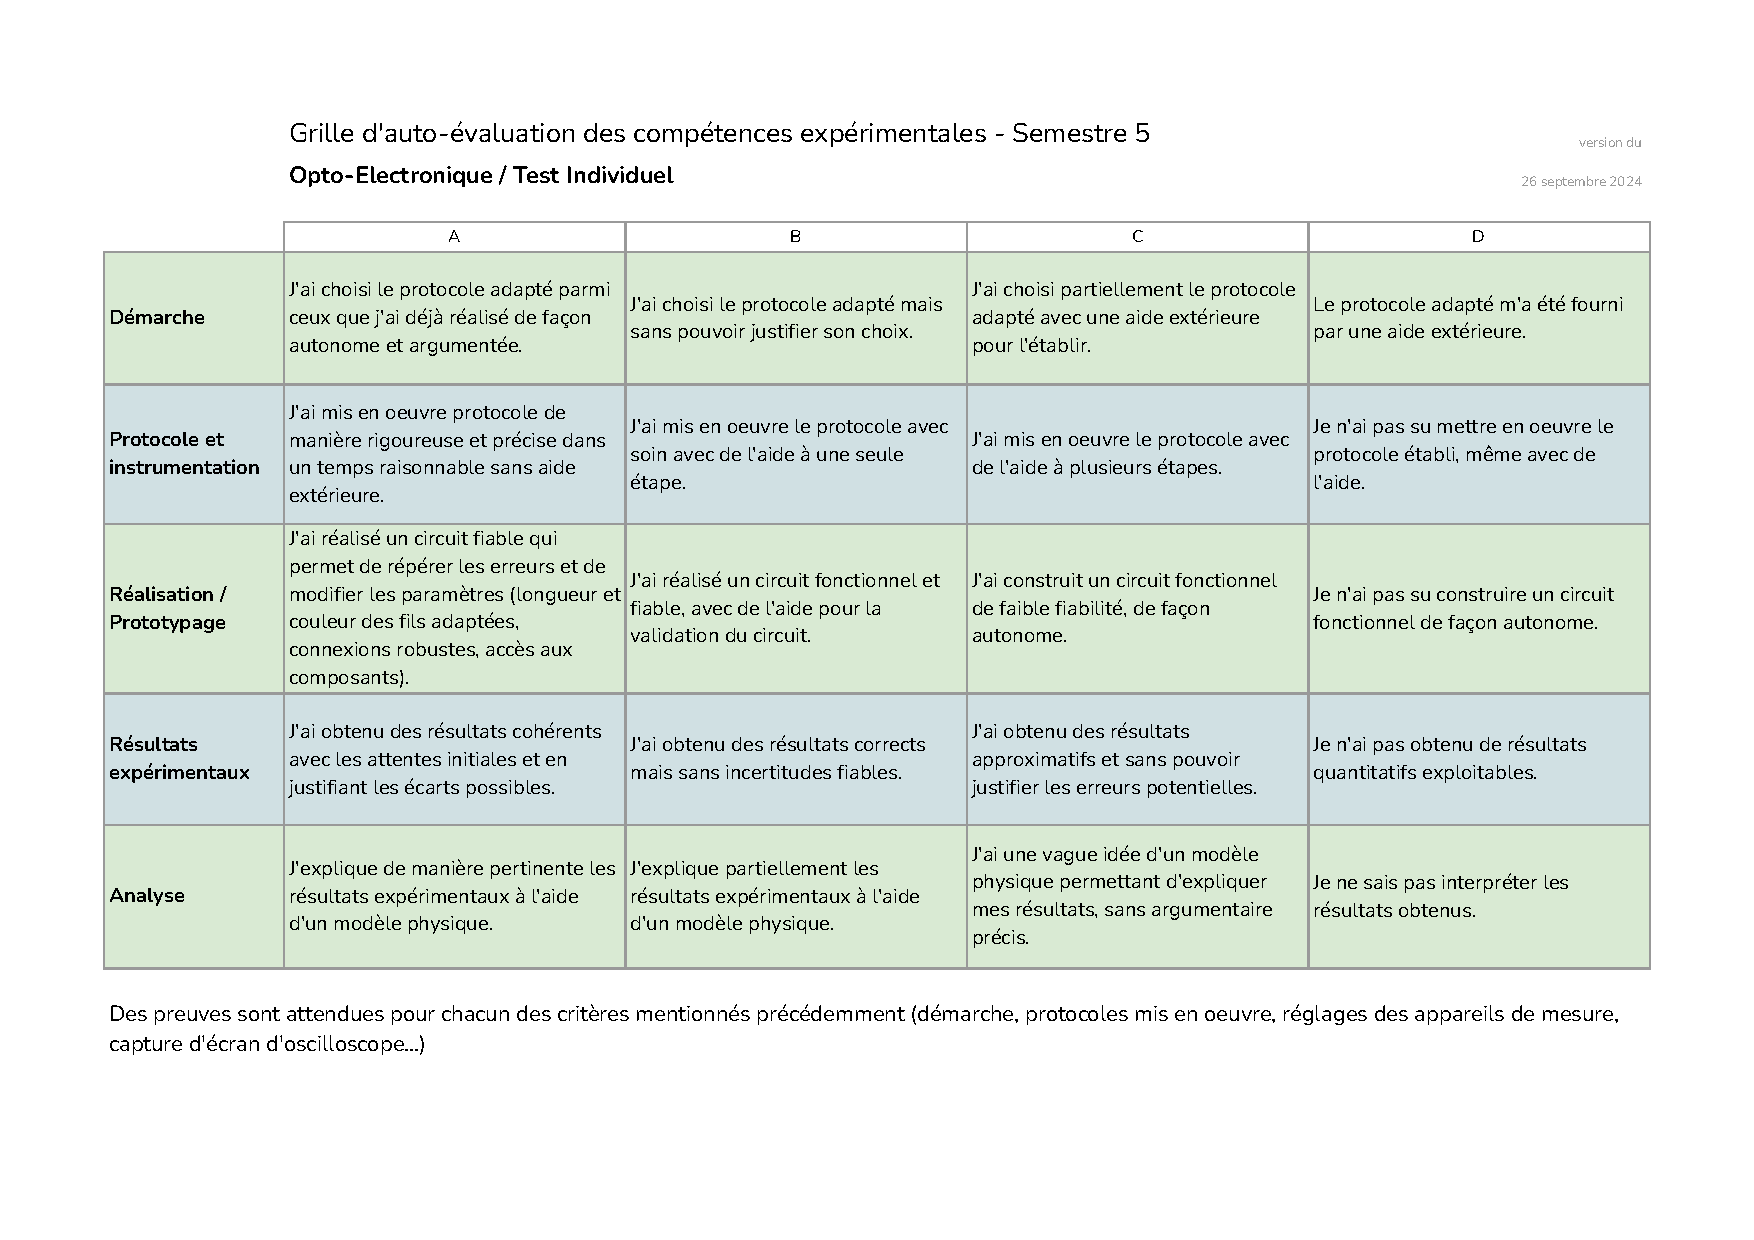
\includepdf[pages=-,landscape=true]{../S5_Optoelectronique_2024_AutoEval_Indiv.pdf}	


\cleardoublepage
%----------------------------------------------------------------------------------------
% SUJET 2
%----------------------------------------------------------------------------------------

	\Large 
\begin{tabular}{c}

\includegraphics[width=5cm]{logoLEnsE.png}
\end{tabular}
\hfill
\begin{tabular}{c}
Travaux Pratiques CéTI \\
Semestre 5 \\
\end{tabular}\\
\normalsize 

\bigskip

\begin{mdframed}[style=aavbox,frametitle={Travail de synthèse}]

L'objectif de l'atelier est de rédiger en temps limité un compte-rendu du travail expérimental accompli dans le cadre du bloc 1 ou du bloc 2. Ce document synthétique et riche de preuves (basées sur vos résultats expérimentaux) a pour objectif de revendiquer le fait que vous êtes capable :

\begin{enumerate}
	\item soit de \textbf{caractériser un dipôle électronique} (linéaire ou non-linéaire) statiquement et en déduire ses zones de fonctionnement, 
	\item soit de \textbf{caractériser un système linéaire} dans les domaines temporel et fréquentiel.
\end{enumerate}

Le livrable de synthèse est évalué en cours de séance par l'encadrant·e. 
\end{mdframed}	

\medskip 

	\noindent \hrulefill
	
	\section*{Partie A / Etude d'un dipôle}
	
	On souhaite caractériser le dipôle mis à votre disposition. 

	\begin{enumerate}
		\item Tracer la caractéristique statique de ce dipôle.
		\item Relever les paramètres importants d'utilisation.
	\end{enumerate}

	\noindent \hrulefill

\textbf{ATTENTION} : Ne dépassez pas un courant de $20\operatorname{mA}$ et une tension inverse de $4\operatorname{V}$ pour le dipôle étudié.

	\noindent \hrulefill
	
	\section*{Partie B / Caractérisation d'un système}
	
	On se propose d'étudier le montage suivant : 
	
	\begin{center}
\begin{circuitikz} 
	\node [op amp, fill=blue!10!white](A1) at (0,0){\texttt{ALI1}};
	\draw (A1.-) to[short] ++(-.5,0) coordinate(A) to[short] ++(0,1.5) coordinate(B) to[R, l^=$R_2$] (B -| A1.out) coordinate(RR) to[short, -*] (A1.out);
	\draw (A1.-) to[short,-*] ++(-.5,0) coordinate(AA) to[R, l_=$R_1$] ++(-2.5,0) coordinate(BB) to [short,l_=${V_e}$, -o] ++(-1,0) coordinate(CC);

	\draw (B) to[short,*-] ++ (0, 1.5) coordinate(RC) to[C, l=$C$] (RC -| A1.out) to[short,-*] (RR);
	\draw (A1.+) to[short] ++(-.5,0) coordinate(AA2) node[cground]{};

	\draw (A1.out) to [short,l=${V_S}$, -o] ++(1,0) coordinate(D);
	
\end{circuitikz}
\end{center}		

\bigskip

Avec $R_1 = 2.2\operatorname{k\Omega}$, $R_2 = 10\operatorname{k\Omega}$ et $C = 100\operatorname{nF}$. L'ALI sera alimenté avec une alimentation symétrique de +/- $12\operatorname{V}$.

\bigskip
	
	\begin{enumerate}
		\item Faire une étude asymptotique en fréquence de ce montage.
		\item Réaliser le montage proposé ci-dessus.
		\item Tracer la \textbf{réponse en fréquence} de ce système et évaluer les \textbf{principales caractéristiques} (gain, bande-passante, ordre, déphasage pour des valeurs pertinentes de fréquence...).
	\end{enumerate}	

	
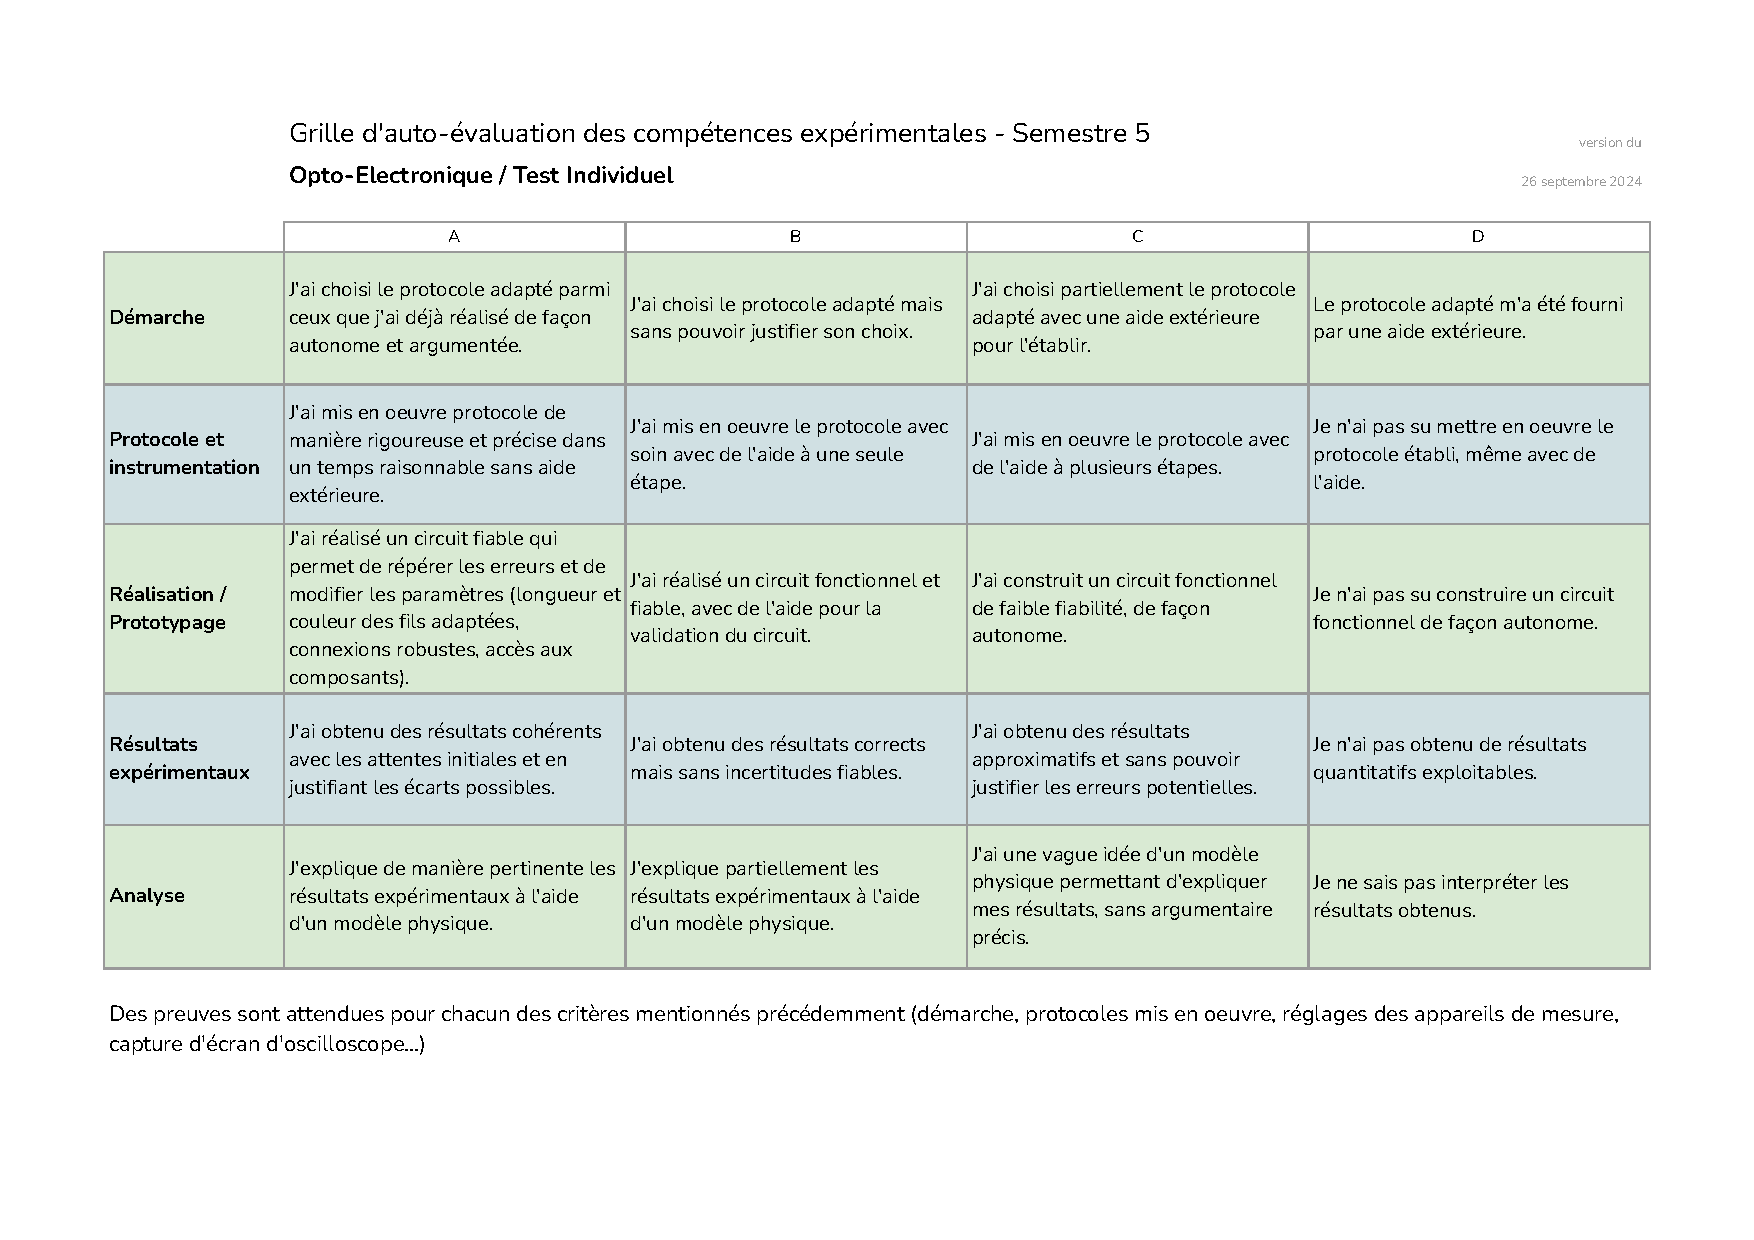
\includepdf[pages=-,landscape=true]{../S5_Optoelectronique_2024_AutoEval_Indiv.pdf}

\cleardoublepage
%----------------------------------------------------------------------------------------
% SUJET 3
%----------------------------------------------------------------------------------------

	\Large 
\begin{tabular}{c}

\includegraphics[width=5cm]{logoLEnsE.png}
\end{tabular}
\hfill
\begin{tabular}{c}
Travaux Pratiques CéTI \\
Semestre 5 \\
\end{tabular}\\
\normalsize 

\bigskip

\begin{mdframed}[style=aavbox,frametitle={Travail de synthèse}]

L'objectif de l'atelier est de rédiger en temps limité un compte-rendu du travail expérimental accompli dans le cadre du bloc 1 ou du bloc 2. Ce document synthétique et riche de preuves (basées sur vos résultats expérimentaux) a pour objectif de revendiquer le fait que vous êtes capable :

\begin{enumerate}
	\item soit de \textbf{caractériser un dipôle électronique} (linéaire ou non-linéaire) statiquement et en déduire ses zones de fonctionnement, 
	\item soit de \textbf{caractériser un système linéaire} dans les domaines temporel et fréquentiel.
\end{enumerate}

Le livrable de synthèse est évalué en cours de séance par l'encadrant·e. 
\end{mdframed}	

\medskip 
	

	\noindent \hrulefill
	
	\section*{Partie A / Etude d'un dipôle}
	
	On souhaite caractériser le dipôle mis à votre disposition.  

	\begin{enumerate}
		\item Tracer la caractéristique statique de ce dipôle.
		\item Relever les paramètres importants d'utilisation.
	\end{enumerate}

	\noindent \hrulefill

\textbf{ATTENTION} : Ne dépassez pas un courant de $20\operatorname{mA}$ et une tension inverse de $4\operatorname{V}$ pour le dipôle étudié.

	\noindent \hrulefill
	
	\section*{Partie B / Caractérisation d'un système}
	
	On se propose d'étudier le montage suivant : 
	
	
	\begin{center}
\begin{circuitikz} 
	\node [op amp, fill=blue!10!white](A1) at (0,0){\texttt{ALI1}};
	\draw (A1.-) to[short] ++(-.5,0) coordinate(A) to[short] ++(0,1.5) coordinate(B) to[R, l^=$R_2$] (B -| A1.out) coordinate(RR) to[short, -*] (A1.out);
	\draw (A1.-) to[short,-*] ++(-.5,0) coordinate(AA) to[R, l_=$R_1$] ++(-2.5,0) coordinate(BB) to [short,l_=${V_e}$, -o] ++(-1,0) coordinate(CC);

	\draw (A1.+) to[short] ++(-.5,0) coordinate(AA2) node[cground]{};

	\draw (A1.out) to [short,l=${V_S}$, -o] ++(1,0) coordinate(D);
	
\end{circuitikz}
\end{center}	

\bigskip

Avec $R_1 = 1\operatorname{k\Omega}$ et $R_2 = 33\operatorname{k\Omega}$. L'ALI sera alimenté avec une alimentation symétrique de +/- $12\operatorname{V}$.
	
\bigskip

	\begin{enumerate}
		\item Faire une étude asymptotique en fréquence de ce montage.
		\item Réaliser le montage proposé ci-dessus.
		\item Tracer la \textbf{réponse en fréquence} de ce système et évaluer les \textbf{principales caractéristiques} (gain, bande-passante, ordre, déphasage pour des valeurs pertinentes de fréquence...).
	\end{enumerate}		
		
	
	
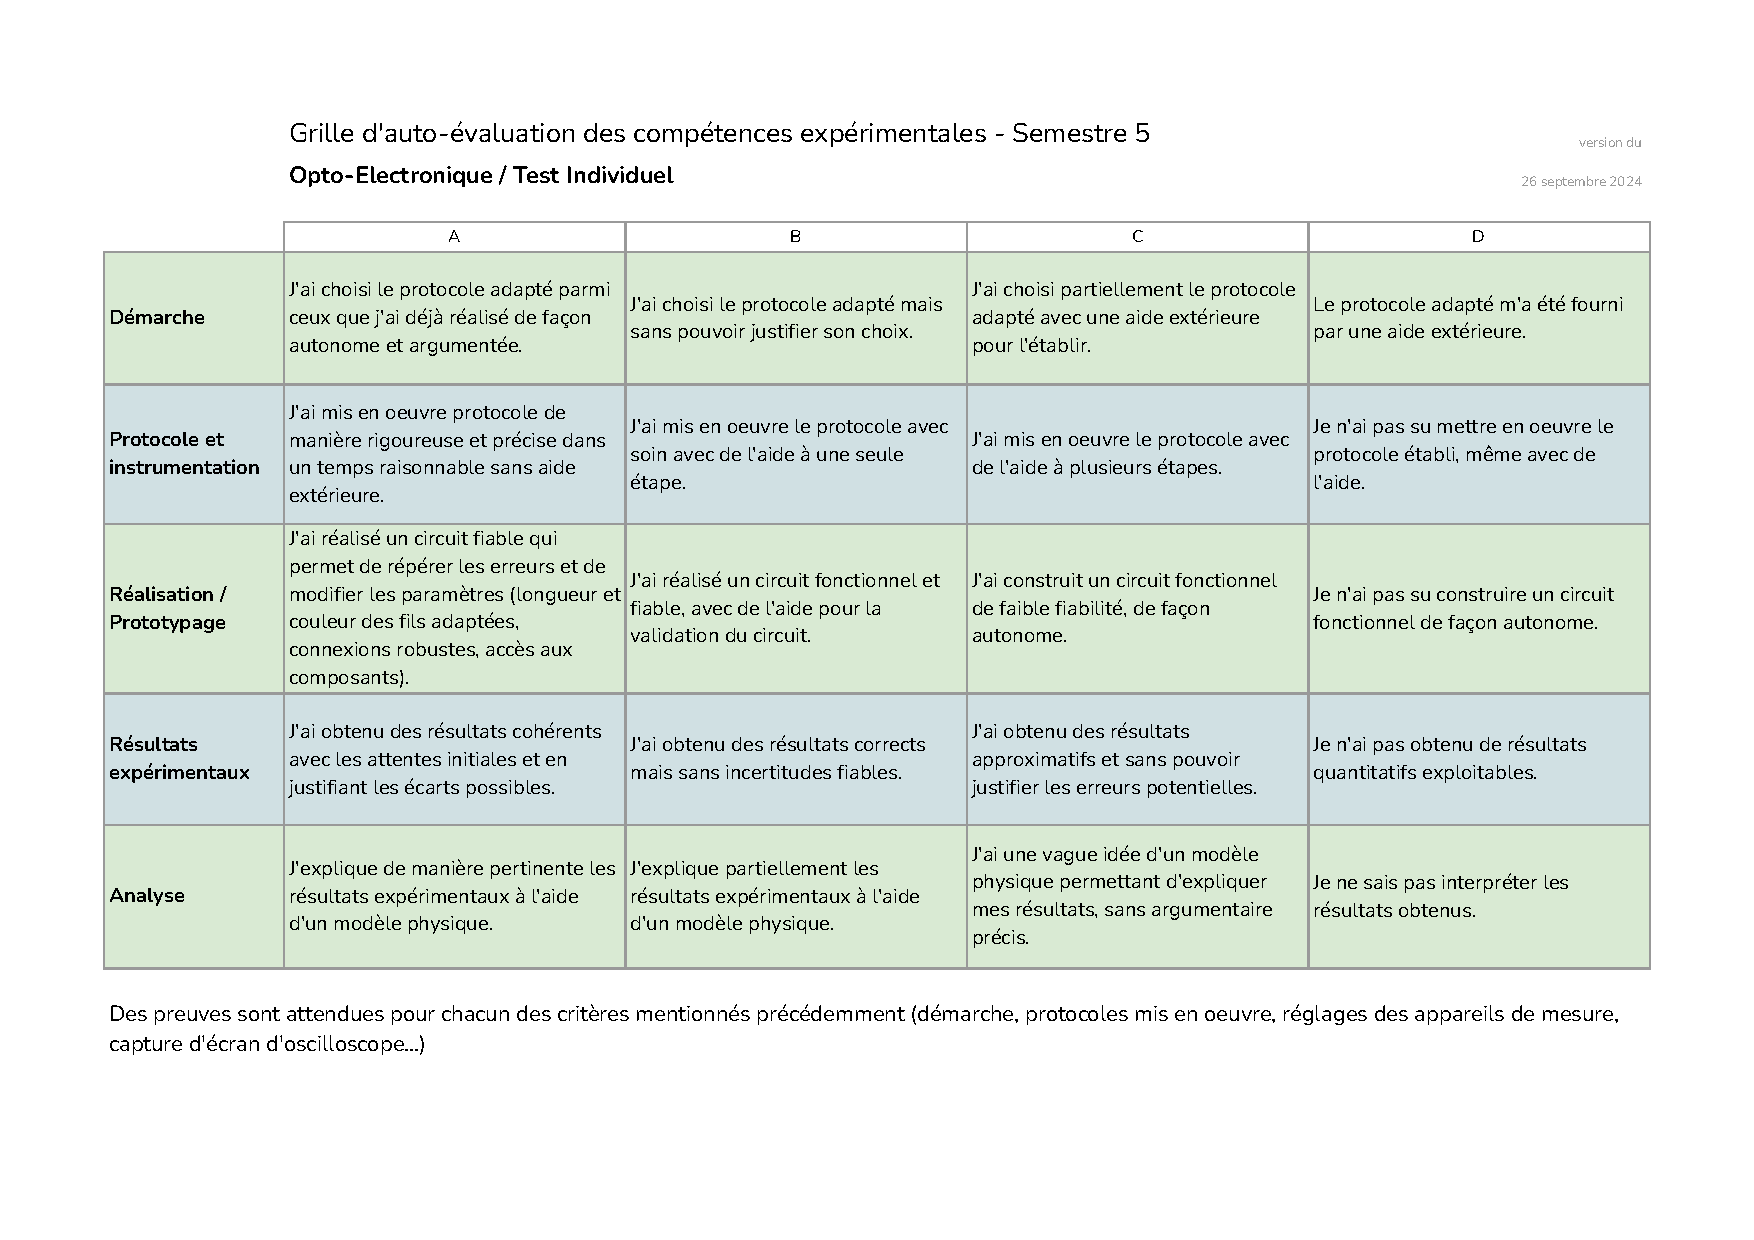
\includepdf[pages=-,landscape=true]{../S5_Optoelectronique_2024_AutoEval_Indiv.pdf}

\cleardoublepage
%----------------------------------------------------------------------------------------
% SUJET 4
%----------------------------------------------------------------------------------------

	\Large 
\begin{tabular}{c}

\includegraphics[width=5cm]{logoLEnsE.png}
\end{tabular}
\hfill
\begin{tabular}{c}
Travaux Pratiques CéTI \\
Semestre 5 \\
\end{tabular}\\
\normalsize 

\bigskip

\begin{mdframed}[style=aavbox,frametitle={Travail de synthèse}]

L'objectif de l'atelier est de rédiger en temps limité un compte-rendu du travail expérimental accompli dans le cadre du bloc 1 ou du bloc 2. Ce document synthétique et riche de preuves (basées sur vos résultats expérimentaux) a pour objectif de revendiquer le fait que vous êtes capable :

\begin{enumerate}
	\item soit de \textbf{caractériser un dipôle électronique} (linéaire ou non-linéaire) statiquement et en déduire ses zones de fonctionnement, 
	\item soit de \textbf{caractériser un système linéaire} dans les domaines temporel et fréquentiel.
\end{enumerate}

Le livrable de synthèse est évalué en cours de séance par l'encadrant·e. 
\end{mdframed}	

\medskip 

	\section*{Partie A / Etude d'un dipôle}
	
	On souhaite caractériser le dipôle mis à votre disposition. 

	\begin{enumerate}
		\item Tracer la caractéristique statique de ce dipôle.
		\item Relever les paramètres importants d'utilisation.
	\end{enumerate}

	\noindent \hrulefill

\textbf{ATTENTION} : Ne dépassez pas un courant de $20\operatorname{mA}$ et une tension inverse de $4\operatorname{V}$ pour le dipôle étudié.

	\noindent \hrulefill
	
	\section*{Partie B / Caractérisation d'un système}

On se propose d'étudier le filtre 2 de la maquette proposée ($IN2$ et $OUT2$).

Il s'agit d'un \textbf{filtre actif} qui nécessite une \textbf{alimentation symétrique} : 
\begin{itemize}
	\item NOIRE : masse
	\item ROUGE : $+V_{CC}$
	\item BLEU : $-V_{CC}$
\end{itemize}

\medskip

\begin{enumerate}
	\item Réaliser l'alimentation symétrique avec $V_{CC} = 12V$.
	\item Alimenter ensuite la maquette.	
	\item Tracer la \textbf{réponse en fréquence} de ce système et évaluer les \textbf{principales caractéristiques} (gain, bande-passante, ordre, déphasage pour des valeurs pertinentes de fréquence...).
\end{enumerate}	

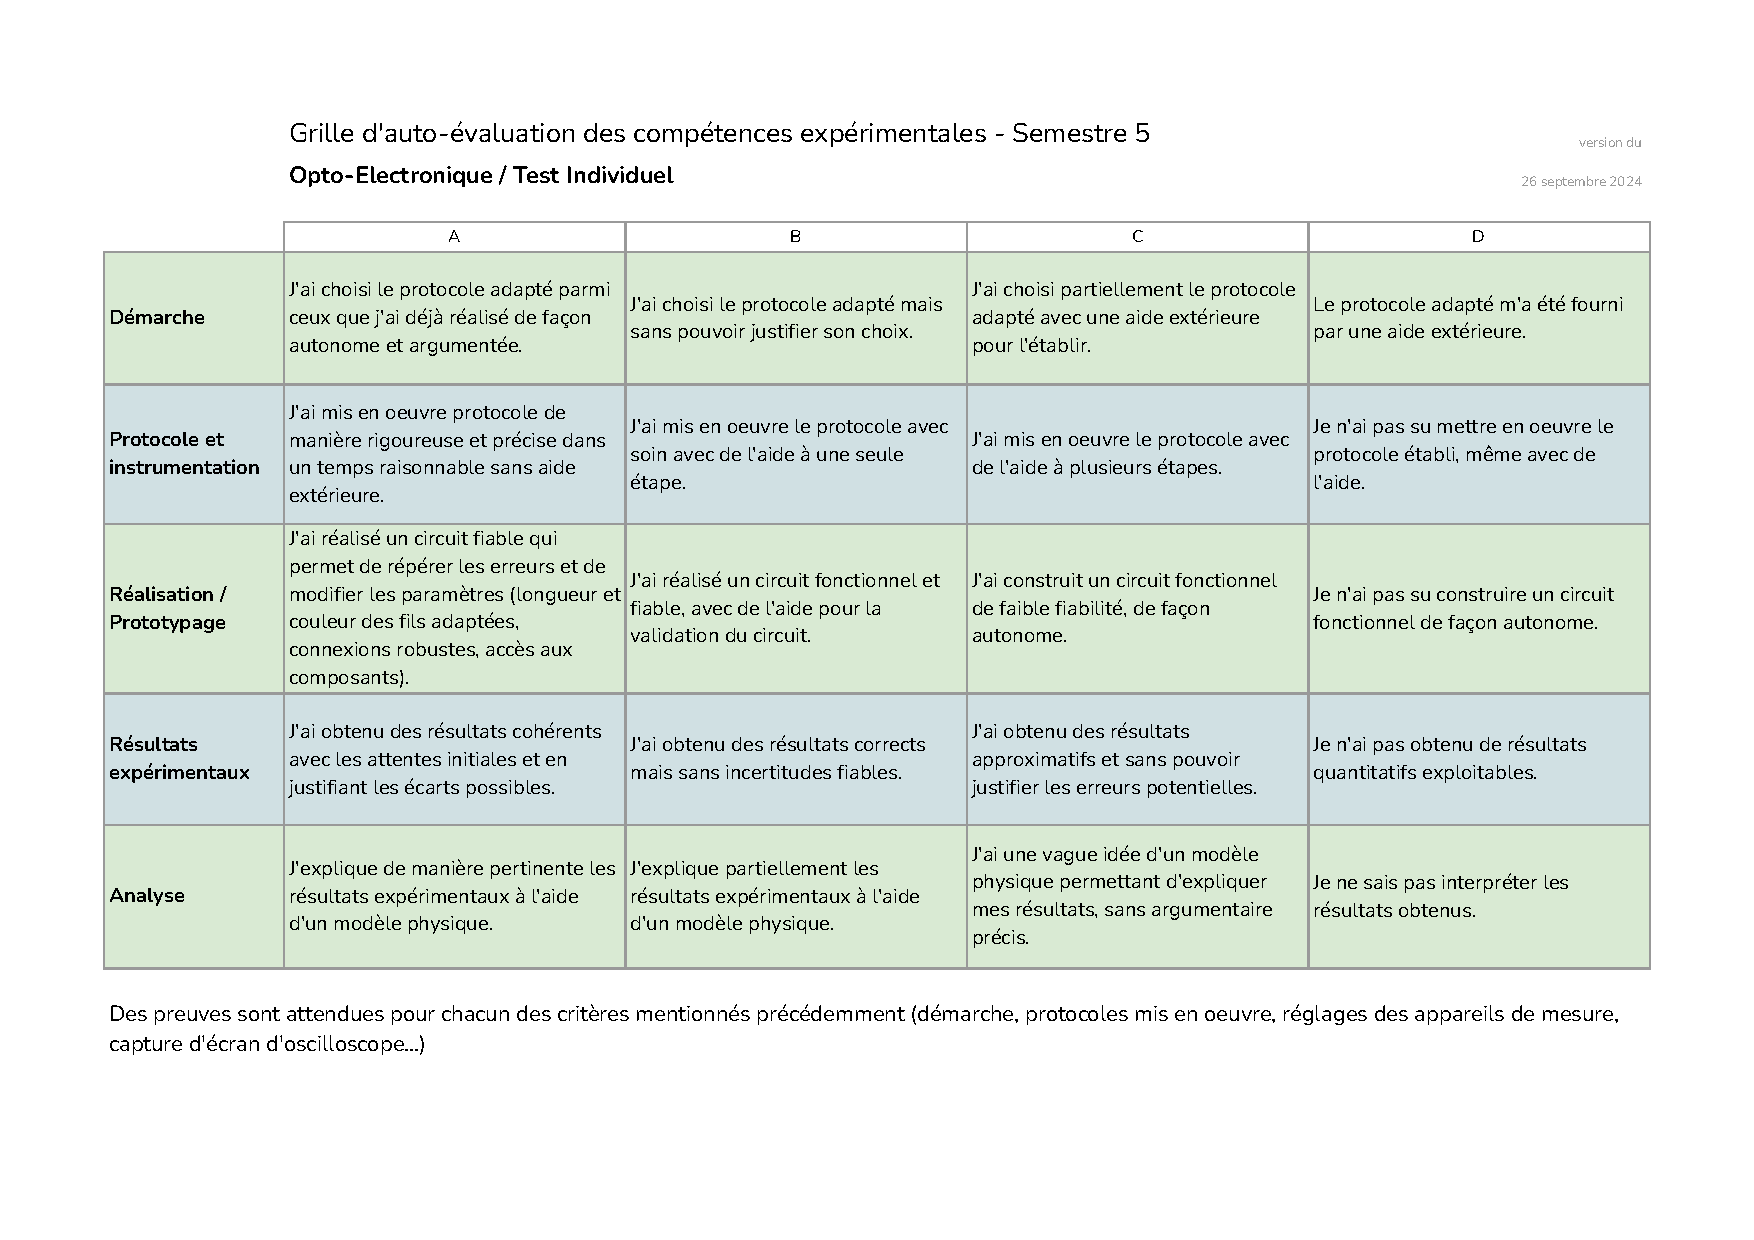
\includepdf[pages=-,landscape=true]{../S5_Optoelectronique_2024_AutoEval_Indiv.pdf}

\end{document}